\section{Background}
\label{chap:background}

\subsection{LUKS2 Disk Encryption}
\label{chap:background.luks2}
\emph{Linux Unified Key Setup 2}, or short LUKS2, is the second version of a disk encryption standard. It provides a specification \cite{Broz2018} for a on-disk format for storing the encryption metadata as well as the encrypted user data. Unlocking an encrypted disk is achieved by providing one of possibly multiple passphrases or keyfiles. The intended usage of LUKS2 is together with the Linux dm-crypt subsystem, but that is not mandatory\footnote{\label{fn:luks2windows} As we show in this thesis, it is possible to make the combination of LUKS2 and Windows work.}.

The differences between the original LUKS and LUKS2 are minor. According to \cite{Broz2018}, LUKS2 adds ``more flexible ways of storing metadata, redundant information to provide recovery in the case of corruption in a metadata area, and an interface to store externally managed metadata for integration with other tools.'' Practically, this means that LUKS2 has a different on-disk layout and, among other things, supports more password hashing algorithms (more precisely, password-based key derivation functions).

The reference implementation\footnote{\label{fn:background.luks2.referenceimpl} \url{https://gitlab.com/cryptsetup/cryptsetup}} is designed only for usage on Linux, which is why we developed a new library in Rust for interacting with LUKS2 partitions. This is not a full equivalent, but only a cross-platform helper. Its task is to take care of all the cryptographic work needed before actually decrypting and encrypting data (more precisely, the process described in \autoref{chap:background.luks2.unlocking}). Notably, it lacks the following features of the reference implementation:
\begin{itemize}[label=\textbf{--}]
	\item formatting new LUKS2 partitions,
	\item modifying or repairing existing LUKS2 partitions,
	\item converting a LUKS partition to a LUKS2 partition,
	\item actually mounting a LUKS2 partition for read/write usage (this is what our kernel driver and its userspace configuration tool is for).
\end{itemize}
Our library does provide access to the raw decrypted user data, but the practical use of this is very limited: the decrypted data is in the format of a filesystem, e.g. FAT32, btrfs, or Ext4. Therefore, a filesystem driver is needed to actually access the stored files. One way of exposing the decrypted data to the system's filesystem drivers is by transparently decrypting the data directly in the kernel, which is what our driver does (see \autoref{chap:ourapproach}).

\subsubsection{On-Disk Format}
\label{chap:background.luks2.ondisk}
\begin{figure}[htb!]
	\begin{tikzpicture}
		\node [anchor=center] at (0.25, 1.5) {\footnotesize\makecell{primary\\binary header}};
		\draw [fill={rgb:black, 1; white, 2}] (0, 0) rectangle (0.5, 1);
		\draw [fill=white] (0.5, 0) rectangle (3.5, 1);
		\node [anchor=center] at (2, 0.5) {\small\makecell{1\textsuperscript{st} JSON area}};
		\node [anchor=center] at (3.75, 1.5) {\footnotesize\makecell{secondary\\binary header}};
		\draw [fill={rgb:black, 1; white, 2}] (3.5, 0) rectangle (4, 1);
		\draw [fill=white] (4, 0) rectangle (7, 1);
		\node [anchor=center] at (5.5, 0.5) {\small\makecell{2\textsuperscript{nd} JSON area}};
		\draw [fill=white] (7, 0) rectangle (10, 1);
		\node [anchor=center] at (8.5, 0.5) {\small\makecell{Keyslots area}};
		\node [anchor=center] at (10.25, 1.5) {\footnotesize\makecell{alignment\\padding}};
		\draw [fill={rgb:black, 1; white, 2}] (10, 0) rectangle (10.5, 1);

		\draw[decorate, decoration={calligraphic brace, amplitude=10pt, mirror}, semithick, yshift=-3pt] (0, 0) -- (10.5, 0) node[midway, yshift=-18pt] {\small Complete header};

		\draw [fill=white] (10.5, 0) rectangle (15, 1);
		\node [anchor=center] at (12.75, 0.5) {\small\makecell{Segment(s)}};
	\end{tikzpicture}
	\caption[
		LUKS2 on-disk format
	]{
		LUKS2 on-disk format (modified after \cite{Broz2018}). The complete header consists of three areas: a binary header of exactly one 4096-byte sector, JSON metadata, and the binary keyslots data. A \emph{keyslot} is an ``encrypted area on disk that contains a key'' \cite{Broz2018}. For redundancy, the binary header and the JSON metadata are stored twice. After that follow one or areas containing encrypted user data. The specification calls these areas \emph{segments}.
	}
	\label{fig:background.luks2.ondisk}
\end{figure}

\autoref{fig:background.luks2.ondisk} shows the high-level layout of a LUKS2-encrypted disk.

The two binary headers have a size of exactly one sector, so that they are always written atomically. Only the first 512 bytes are actually used. The header marks the disk as following the LUKS2 specification, and contains metadata such as labels, a UUID, and a header checksum. The labels and UUID can be accessed using the \texttt{blkid}\footnote{\label{fn:background.luks2.blkid} \url{https://linux.die.net/man/8/blkid}} command-line tool and also be used in the \texttt{udev}\footnote{\label{fn:background.luks2.udev} \url{https://linux.die.net/man/8/udev}} Linux subsystem. For the detailed contents, see \autoref{fig:background.luks2.binhdrstructure}. \autoref{fig:background.luks2.binhdrexample} also contains an example hexdump of a binary header.

\begin{figure}[htb!]
	\begin{ccode}
#define MAGIC_1ST "LUKS\xba\xbe"
#define MAGIC_2ND "SKUL\xba\xbe"
#define MAGIC_L     6
#define UUID_L     40
#define LABEL_L    48
#define SALT_L     64
#define CSUM_ALG_L 32
#define CSUM_L     64

struct luks2_hdr_disk {
    char     magic[MAGIC_L];       // MAGIC_1ST or MAGIC_2ND
    uint16_t version;              // Version 2
    uint64_t hdr_size;             // size including JSON area [bytes]
    uint64_t seqid;                // sequence ID, increased on update
    char     label[LABEL_L];       // ASCII label or empty
    char     csum_alg[CSUM_ALG_L]; // checksum algorithm, "sha256"
    uint8_t  salt[SALT_L];         // salt, unique for every header
    char     uuid[UUID_L];         // UUID of device
    char     subsystem[LABEL_L];   // owner subsystem label or empty
    uint64_t hdr_offset;           // offset from device start [bytes]
    char    _padding[184];         // must be zeroed
    uint8_t  csum[CSUM_L];         // header checksum
    char    _padding4096[7*512];   // Padding, must be zeroed
} __attribute__((packed));
	\end{ccode}
	\caption[
		LUKS2 binary header structure
	]{
		LUKS2 binary header structure from \cite{Broz2018}. Integers are stored in big-endian format, and all strings have to be null-terminated. The \texttt{magic}, \texttt{version}, and \texttt{uuid} fields are also present in the LUKS1 binary header and were placed at the same offsets as there.
	}
	\label{fig:background.luks2.binhdrstructure}
\end{figure}

\begin{figure}[htb!]
	\ttfamily
	\scriptsize
	\begin{NiceTabular}{c|*{16}{c}|l}
	\CodeBefore
		\rectanglecolor{tPink}{1-2}{1-7}    \rectanglecolor{tOrng}{1-8}{1-9}     \rectanglecolor{tYlow}{1-10}{1-17}
		\rectanglecolor{tGren}{2-2}{2-9}    \rectanglecolor{tLblu}{2-10}{2-17}
		\rectanglecolor{tLblu}{3-2}{3-17}
		\rectanglecolor{tLblu}{4-2}{4-17}
		\rectanglecolor{tLblu}{5-2}{5-9}    \rectanglecolor{tBlue}{5-10}{5-17}
		\rectanglecolor{tBlue}{6-2}{6-17}
		\rectanglecolor{tBlue}{7-2}{7-9}    \rectanglecolor{tPurp}{7-10}{7-17}
		\rectanglecolor{tPurp}{8-2}{8-17}
		\rectanglecolor{tPurp}{9-2}{9-17}
		\rectanglecolor{tPurp}{10-2}{10-17}
		\rectanglecolor{tPurp}{11-2}{11-9}  \rectanglecolor{tRose}{11-10}{11-17}
		\rectanglecolor{tRose}{12-2}{12-17}
		\rectanglecolor{tRose}{13-2}{13-17}
		\rectanglecolor{tPink}{14-2}{14-17}
		\rectanglecolor{tPink}{15-2}{15-17}
		\rectanglecolor{tPink}{16-2}{16-17}
		\rectanglecolor{tOrng}{17-2}{17-9}  \rectanglecolor{tYlow}{17-10}{17-17}
		\rectanglecolor{tYlow}{18-2}{18-17}
		\rectanglecolor{tYlow}{19-2}{19-17}
		\rectanglecolor{tYlow}{20-2}{20-17}
		\rectanglecolor{tYlow}{21-2}{21-17}
		\rectanglecolor{tYlow}{22-2}{22-17}
		\rectanglecolor{tYlow}{23-2}{23-17}
		\rectanglecolor{tYlow}{24-2}{24-17}
		\rectanglecolor{tYlow}{25-2}{25-17}
		\rectanglecolor{tYlow}{26-2}{26-17}
		\rectanglecolor{tYlow}{27-2}{27-17}
		\rectanglecolor{tYlow}{28-2}{28-17}
		\rectanglecolor{tGren}{29-2}{29-17}
		\rectanglecolor{tGren}{30-2}{30-17}
		\rectanglecolor{tGren}{31-2}{31-17}
		\rectanglecolor{tGren}{32-2}{32-17}
	\Body
	    0000 & 4C & 55 & 4B & 53 & BA & BE & 00 & 02 & 00 & 00 & 00 & 00 & 00 & 00 & 40 & 00 & \coltxt{tPink}{LUKSº¾}\coltxt{tOrng}{..}\coltxt{tYlow}{......@.} \\
        0010 & 00 & 00 & 00 & 00 & 00 & 00 & 00 & 03 & 54 & 68 & 69 & 73 & 20 & 69 & 73 & 20 & \coltxt{tGren}{........}\coltxt{tLblu}{This is } \\
        0020 & 61 & 6E & 20 & 41 & 53 & 43 & 49 & 49 & 20 & 6C & 61 & 62 & 65 & 6C & 00 & 00 & \coltxt{tLblu}{an ASCII label..} \\
        0030 & 00 & 00 & 00 & 00 & 00 & 00 & 00 & 00 & 00 & 00 & 00 & 00 & 00 & 00 & 00 & 00 & \coltxt{tLblu}{................} \\
        0040 & 00 & 00 & 00 & 00 & 00 & 00 & 00 & 00 & 73 & 68 & 61 & 32 & 35 & 36 & 00 & 00 & \coltxt{tLblu}{........}\coltxt{tBlue}{sha256..} \\
        0050 & 00 & 00 & 00 & 00 & 00 & 00 & 00 & 00 & 00 & 00 & 00 & 00 & 00 & 00 & 00 & 00 & \coltxt{tBlue}{................} \\
        0060 & 00 & 00 & 00 & 00 & 00 & 00 & 00 & 00 & EB & 0F & D2 & C6 & E3 & D2 & 8D & 4B & \coltxt{tBlue}{........}\coltxt{tPurp}{ë.ÒÆãÒ.K} \\
        0070 & BB & 2B & 8A & 49 & E6 & 2E & 4E & B7 & 04 & 2F & A9 & 39 & 76 & 71 & 8F & 8A & \coltxt{tPurp}{»+ŠIæ.N·./©9vq.Š} \\
        0080 & 33 & E8 & F3 & 90 & FF & DC & 4D & 3D & E8 & 30 & 7B & 37 & 01 & 30 & E7 & 5D & \coltxt{tPurp}{3èó.ÿÜM=è0\{7.0ç]} \\
        0090 & AD & A0 & 57 & 1C & 0E & 63 & BC & D4 & DD & 3C & EC & F5 & DE & 67 & F8 & D8 & \coltxt{tPurp}{..W..c¼ÔÝ<ìõÞgøØ} \\
        00A0 & F2 & 7E & 82 & CD & B9 & DD & 77 & 10 & 65 & 39 & 33 & 64 & 63 & 61 & 66 & 61 & \coltxt{tPurp}{ò\nicetilde{}‚͹Ýw.}\coltxt{tRose}{e93dcafa} \\
        00B0 & 2D & 65 & 65 & 30 & 62 & 2D & 34 & 31 & 36 & 38 & 2D & 61 & 61 & 37 & 63 & 2D & \coltxt{tRose}{-ee0b-4168-aa7c-} \\
        00C0 & 66 & 33 & 30 & 34 & 37 & 34 & 38 & 38 & 36 & 61 & 32 & 65 & 00 & 00 & 00 & 00 & \coltxt{tRose}{f30474886a2e....} \\
        00D0 & 54 & 68 & 69 & 73 & 20 & 69 & 73 & 20 & 61 & 6E & 20 & 6F & 70 & 74 & 69 & 6F & \coltxt{tPink}{This is an optio} \\
        00E0 & 6E & 61 & 6C & 20 & 73 & 65 & 63 & 6F & 6E & 64 & 61 & 72 & 79 & 20 & 6C & 61 & \coltxt{tPink}{nal secondary la} \\
        00F0 & 62 & 65 & 6C & 00 & 00 & 00 & 00 & 00 & 00 & 00 & 00 & 00 & 00 & 00 & 00 & 00 & \coltxt{tPink}{bel.............} \\
        0100 & 00 & 00 & 00 & 00 & 00 & 00 & 00 & 00 & 00 & 00 & 00 & 00 & 00 & 00 & 00 & 00 & \coltxt{tOrng}{........}\coltxt{tYlow}{........} \\
        0110 & 00 & 00 & 00 & 00 & 00 & 00 & 00 & 00 & 00 & 00 & 00 & 00 & 00 & 00 & 00 & 00 & \coltxt{tYlow}{................} \\
        0120 & 00 & 00 & 00 & 00 & 00 & 00 & 00 & 00 & 00 & 00 & 00 & 00 & 00 & 00 & 00 & 00 & \coltxt{tYlow}{................} \\
        0130 & 00 & 00 & 00 & 00 & 00 & 00 & 00 & 00 & 00 & 00 & 00 & 00 & 00 & 00 & 00 & 00 & \coltxt{tYlow}{................} \\
        0140 & 00 & 00 & 00 & 00 & 00 & 00 & 00 & 00 & 00 & 00 & 00 & 00 & 00 & 00 & 00 & 00 & \coltxt{tYlow}{................} \\
        0150 & 00 & 00 & 00 & 00 & 00 & 00 & 00 & 00 & 00 & 00 & 00 & 00 & 00 & 00 & 00 & 00 & \coltxt{tYlow}{................} \\
        0160 & 00 & 00 & 00 & 00 & 00 & 00 & 00 & 00 & 00 & 00 & 00 & 00 & 00 & 00 & 00 & 00 & \coltxt{tYlow}{................} \\
        0170 & 00 & 00 & 00 & 00 & 00 & 00 & 00 & 00 & 00 & 00 & 00 & 00 & 00 & 00 & 00 & 00 & \coltxt{tYlow}{................} \\
        0180 & 00 & 00 & 00 & 00 & 00 & 00 & 00 & 00 & 00 & 00 & 00 & 00 & 00 & 00 & 00 & 00 & \coltxt{tYlow}{................} \\
        0190 & 00 & 00 & 00 & 00 & 00 & 00 & 00 & 00 & 00 & 00 & 00 & 00 & 00 & 00 & 00 & 00 & \coltxt{tYlow}{................} \\
        01A0 & 00 & 00 & 00 & 00 & 00 & 00 & 00 & 00 & 00 & 00 & 00 & 00 & 00 & 00 & 00 & 00 & \coltxt{tYlow}{................} \\
        01B0 & 00 & 00 & 00 & 00 & 00 & 00 & 00 & 00 & 00 & 00 & 00 & 00 & 00 & 00 & 00 & 00 & \coltxt{tYlow}{................} \\
        01C0 & 91 & A4 & A9 & 83 & 03 & FF & FB & 68 & 4E & C2 & 94 & 6F & 4C & 78 & 71 & AF & \coltxt{tGren}{‘¤©ƒ.ÿûhN”oLxq¯} \\
        01D0 & AE & 1A & 91 & F8 & E0 & 2C & F3 & 71 & D5 & 17 & CB & 60 & E5 & 2F & D6 & 36 & \coltxt{tGren}{®.‘øà,óqÕ.Ë`å/Ö6} \\
        01E0 & 00 & 00 & 00 & 00 & 00 & 00 & 00 & 00 & 00 & 00 & 00 & 00 & 00 & 00 & 00 & 00 & \coltxt{tGren}{................} \\
        01F0 & 00 & 00 & 00 & 00 & 00 & 00 & 00 & 00 & 00 & 00 & 00 & 00 & 00 & 00 & 00 & 00 & \coltxt{tGren}{................}
	\end{NiceTabular}
	\caption[
		LUKS2 binary header example
	]{
		LUKS2 binary header example. The fields, as described in \autoref{fig:background.luks2.binhdrstructure}, were coloured differently to be easily distinguishable. A similar header, although with different salt and hash, can be generated by executing \texttt{fallocate -l 16M luks2.img \&\& cryptsetup luksFormat ---label 'This is an ASCII label' ---subsystem 'This is an optional secondary label' ---uuid e93dcafa-ee0b-4168-aa7c-f30474886a2e luks2.img} in a Linux shell.
	}
	\label{fig:background.luks2.binhdrexample}
\end{figure}

The sector containing the binary header is followed by the JSON area. This area contains the metadata that is arguably most relevant for decryption and encryption. \autoref{fig:background.luks2.jsonobjects} contains an overview of the objects stored in JSON and their relationships. For this thesis' brevity's sake, please refer to chapter 3.1 in \cite{Broz2018} for an example of a LUKS2 JSON area.

\begin{figure}[htb!]
	\center
	\begin{tikzpicture}
		\node       (pass) at (4, 3.5)  {\small Passphrase};
		\node       (stor) at (8, 3.5)  {\small External Keystore};
		\node[rect] (dgst) at (0, 1.75) {\small Digest};
		\node[rect] (kslt) at (4, 1.75) {\small Keyslot};
		\node[rect] (tokn) at (8, 1.75) {\small Token};
		\node[rect] (conf) at (0, 0)    {\small Config};
		\node[rect] (segm) at (4, 0)    {\small Segment};

		\draw (pass) edge[arrow] (kslt);
		\draw (stor) edge[arrow] (tokn);

		\draw (dgst) edge[arrow] node[anchor=south, yshift=-4pt] {\small\makecell{validates}}   (kslt);
		\draw (tokn) edge[arrow] node[anchor=south, yshift=-4pt] {\small\makecell{can open}}    (kslt);
		\draw (kslt) edge[arrow] node[anchor=west]               {\small\makecell{is used for}} (segm);
	\end{tikzpicture}
	\caption[
		LUKS2 object schema
	]{
		LUKS2 object schema from \cite{Broz2018}. The most important objects are the following: \emph{keyslots}, which describe the details of how cryptographic keys are stored and encrypted; \emph{digests}, which can be used to verify that one has successfully extracted a key from a keyslot; and \emph{segments}, which describe the disk areas where the encrypted user data is stored. \autoref{fig:background.luks2.ondisk} shows where the areas described by the keyslot and segment objects actually lie on disk.
	}
	\label{fig:background.luks2.jsonobjects}
\end{figure}

After the JSON area, the keyslots area is stored on the disk. This is space reserved for storing encrypted cryptographic keys. The metadata from the JSON keyslot objects describe the position of a key on the disk as well as information on how to decrypt it. 

\subsubsection{Unlocking a Partition}
\label{chap:background.luks2.unlocking}
For simplicity, our LUKS2 Rust library does not support unlocking a keyslot using an external keystore defined by a token, even though \autoref{fig:background.luks2.jsonobjects} mentions this possibility. Only unlocking via password is implemented. The library does however include support for different \emph{password-based key derivation functions (PBKDFs)}, namely \texttt{pbkdf2} with SHA-256, \texttt{argon2i}, and \texttt{argon2id}. These are all the PBKDF algorithms that are listed in the LUKS2 specification (see \cite{Broz2018}, Table 3). The default PBKDF used by LUKS2 is \texttt{argon2i} \cite{Cryptsetup2020}. In the following paragraphs, it will become apparent what PBKDFs are used for in LUKS2\footnote{\label{fn:background.luks2.pbkdfs} It will also become apparent that they are quite aptly named.}.

The LUKS2 specification allows for multiple segments in one partition. To make things easier, our driver only supports unlocking one segment. Therefore, in this thesis we may speak of unlocking a partition and mean unlocking one of the partition's segments.

To unlock a segment means to derive the cryptographic key that is needed for reading decrypted or writing encrypted data. This key is called the segment's \emph{master key}.

LUKS2 uses a process called \emph{anti-forensic splitting} to store the master key on disk. This method was introduced in \cite{Fruhwirth2005}. It is used to diffuse the key's bytes into a longer sequence of bytes that has the following property: if at least one bit of the diffused sequence is changed, the key cannot be recovered. This is achieved by a clever combination of XOR and a hash function. The motivation behind this to make it easier (or possible) to dispose of an old key in such a way that it cannot be recovered from the disk. This is because it is much more feasible to partially erase a long sequence of bytes than to completely erase a short sequence. Erasing here means to overwrite the data in such a way that it cannot be recovered, which is not as trivial as one might think.

\cite{Fruhwirth2005} calls the operation that splits data anti-forensically AFsplit and the recovery operation AFmerge. We will adhere to this convention (with slight variations).

To necessitate the need of a password to recover the key, the data is also encrypted before it gets written to the disk. The encryption key is a hash of the password obtained by a PBKDF.

The properties of anti-forensic splitting can be used when the user wants to change the password: the master key is derived using the old password and then re-encrypted with the new password. The key as it was encrypted with the old password can then be destroyed.

\cite{Fruhwirth2005} presents two templates for storing keys, TKS1 and TKS2. The difference is whether the key is encrypted before or after splitting it. LUKS and LUKS2 use TKS2, which is schematically explained in \autoref{fig:background.luks2.tks2}. The hash function used by LUKS2 for anti-forensic splitting is SHA-256. \autoref{fig:background.luks2.masterkeydecrypt} shows the outline of an implementation of TKS2 in Rust.

\begin{figure}[htb!]
	\center
	\begin{tikzpicture}
		\node[rect, anchor=east] (pbkdf) at (8, 4) {\small PBKDF2};
		\node[rect]              (ciphr) at (3, 2) {\small Cipher};
		\node[rect, anchor=west] (merge) at (8, 2) {\small AF-merge};
		\node[rect, anchor=east] (rtcip) at (8, -0.5) {\small Real time cipher};

		\draw[arrow] (ciphr)                   -- node[anchor=south, yshift=-4pt] {\small\makecell{Split master key}}  (merge);
		\draw[arrow] (pbkdf.west)  + (-2.5, 0) -- node[anchor=south, yshift=-4pt] {\small\makecell{Passphrase}}          (pbkdf.west);
		\draw[arrow] (pbkdf.north) + (-0.6, 1) -- node[anchor=west]               {\small\makecell{Salt}}                +(-0.6, 0);
		\draw[arrow] (pbkdf.north) + (0.6,  1) -- node[anchor=west]               {\small\makecell{Hash iteration rate}} +(0.6,  0);
		\draw[arrow] (ciphr.west)  + (-2.5, 0) -- node[anchor=south, yshift=-4pt] {\small\makecell{Key storage}}         (ciphr.west);
		\draw[arrow] (rtcip.west)  + (-4,   0) -- node[anchor=south, yshift=-4pt] {\small\makecell{Encrypted partition}} (rtcip.west);
		\draw[arrow] (rtcip.east)              -- node[anchor=south, yshift=-4pt] {\small\makecell{Recovered partition}} +(4,    0);

		\draw[arrow] (pbkdf.east) -- +(1, 0) -- +(1, -1) -| (ciphr.north);
		\draw[arrow] (merge.east) -- +(1, 0) -- +(1, -1) -| node[anchor=east, yshift=-1.2em] {\small\makecell{Master key}} (rtcip.north);
	\end{tikzpicture}
	\caption[
		TKS2 scheme
	]{
		TKS2 scheme (modified after \cite{Fruhwirth2005}).
	}
	\label{fig:background.luks2.tks2}
\end{figure}

\begin{figure}[htb!]
	\begin{rustcode}
fn decrypt_keyslot(
	password: &[u8], keyslot: &LuksKeyslot, json: &LuksJson, /* ... */
) -> Result<Vec<u8>, LuksError> {
	let mut k = vec![
		0; keyslot.key_size() as usize * keyslot.af.stripes() as usize
	];
	// read keyslot data from disk into k...

	let mut pw_hash = vec![0; area.key_size() as usize];
	match keyslot.kdf() {
		// hash into pw_hash using pbkdf2, argon2i, or argon2id...
	}

	// decrypt keyslot area using the password hash as key
	match area.key_size() {
		32 => {
			let key1 = Aes128::new_varkey(&pw_hash[..16]).unwrap();
			let key2 = Aes128::new_varkey(&pw_hash[16..]).unwrap();
			let xts = Xts128::<Aes128>::new(key1, key2);
			xts.decrypt_area(&mut k, sector_size, 0, get_tweak_default);
		},
		// 64 byte key uses AES256 instead...
	}

	// merge and hash master key
	let master_key = af::merge(
		&k, keyslot.key_size() as usize, af.stripes() as usize
	);
	let digest_actual = base64::decode(json.digests[&0].digest())?;
	let mut digest_computed = vec![0; digest_actual.len()];
	let salt = base64::decode(json.digests[&0].salt())?;
	pbkdf2::pbkdf2::<Hmac<Sha256>>(
		&master_key, &salt, json.digests[&0].iterations(), &mut digest_computed
	);

	// compare digests
	if digest_computed == digest_actual {
		Ok(master_key)
	} else {
		Err(LuksError::InvalidPassword)
	}
}
	\end{rustcode}
	\caption[
		LUKS2 master key decryption in Rust
	]{
		LUKS2 master key decryption in Rust. Some values are hardcoded: only the digest with index 0 is used (lines 29, 31, 33), and it is assumed that the digest algorithm is always \texttt{pbkdf2} with SHA-256 (line 32). The latter is compliant with the specification, which lists this digest algorithm as the only option, but not optimal in the sense of input validation.
	}
	\label{fig:background.luks2.masterkeydecrypt}
\end{figure}

The keyslots area on the disk is large enough to store multiple split and encrypted master keys. Thus one can configure a LUKS2 partition to be unlocked by different passwords. Unlocking then works as described in \autoref{fig:background.luks2.unlocking}.

\begin{figure}[htb!]
	\center
	\begin{mdframed}
		\begin{enumerate}
			\item The user supplies a password.
			\item One of the available keyslots is selected.
			\item Using the password and keyslot, the master key is decrypted as described above.
			\item The derived master key is hashed and the result compared to the corresponding digest. Which digest and what hash parameters to used is defined in the JSON section.
			\item If the digests match, the master key has been successfully decrypted. Else go to step 2 and select a keyslot that has not been used yet.
			\item If the master key could not be decrypted with all available keyslots, the supplied password was not correct.
		\end{enumerate}
	\end{mdframed}
	\caption[
		LUKS2 master key decryption with multiple available keyslots
	]{
		LUKS2 master key decryption with multiple available keyslots. LUKS2 also allows defining priorities that govern the order in which the available keyslots are tried. For a more detailed pseudocode see Figure 5 in \cite{Fruwirth2018}.
	}
	\label{fig:background.luks2.unlocking}
\end{figure}

\subsubsection{Using an Unlocked Partition}
\label{chap:background.luks2.using}
After a partition has been unlocked, i.e. after the master key of one of its segments has been decrypted, the partition is ready to be read from and written to. This happens using what \autoref{fig:background.luks2.tks2} calls a real time cipher. LUKS2 supports different encryption algorithms for this purpose, see \autoref{tbl:background.luks2.encryptionalgorithms} for a selection of them. Our driver only supports the default aes-xts-plain64 encryption. Therefore, we will focus on that in this section.

\begin{table}[htb!]
	\center
	\def\arraystretch{1.25}
	\begin{NiceTabular}{cc}
	\CodeBefore
		\rectanglecolor{gray!30}{1-1}{2-2}
	\Body
		\hlineB{2}
		\textbf{Algorithm}            & \textbf{Description} \\
		in \texttt{dm-crypt} notation &                      \\
		\hlineB{1.5}
		aes-xts-plain64      & \makecell{AES in XTS mode with sequential IV} \\
		aes-cbc-essiv:sha256 & \makecell{AES in CBC mode with ESSIV IV}      \\
		serpent-xts-plain64  & \makecell{Serpent cipher with sequential IV}  \\
		twofish-xts-plain64  & \makecell{Twofish cipher with sequential IV}  \\
		\hlineB{2}
	\end{NiceTabular}
	\caption[
		Selection of LUKS2 encryption algorithms
	]{
		Selection of LUKS2 encryption algorithms (modified after \cite{Broz2018}). The \texttt{dm-crypt} algorithm notation is described in \autoref{chap:otherapproaches.linux.dm}. See \cite{Ferguson2010} for the CBC mode and the Serpent and Twofish ciphers, and \cite{Fruhwirth2005} for the ESSIV IV mode.
	}
	\label{tbl:background.luks2.encryptionalgorithms}
\end{table}

The AES encryption algorithm is a block cipher for processing 128 bit data blocks \cite{Fips197}. This means that AES takes a key and 128 bits, or 16 bytes, of data, and generates 16 bytes of encrypted data, called ciphertext. Using the same key, this ciphertext can be decrypted back to the original plaintext data. The key can be 128, 192, or 256 bits long. The three variants of AES, each using a different key size, are called AES-128, AES-192, and AES-256.

To encrypt data longer than one block, a \emph{block cipher mode} is needed \cite{Ferguson2010}. These are encryption functions that build on a existing block cipher. When using aes-xts-plain64, LUKS2 uses the XTS block cipher mode. The defining IEEE standard \cite{Ieee2019} describes it as follows: ``XTS-AES is a tweakable block cipher that acts on data units of 128 b[its] or more and uses the AES block cipher as a subroutine. The key material for XTS-AES consists of a data encryption key (used by the AES block cipher) as well as a `tweak key' that is used to incorporate the logical position of the data block into the encryption.'' This tweak key is called the \emph{initialization vector}, or IV, in the context of LUKS2. This is what the ``plain64'' in aes-xts-plain64 means: ``the initial vector is the 64-bit little-endian version of the sector number, padded with zeros if necessary'' \cite{Dmcrypt2020}. This sector number is relative to the first sector of the segment, i.e. the first sector uses an IV of 0.

The need for an IV arises from a critical problem that occurs when encrypting each block separately with the same key: if some unencrypted blocks are identical, then so will be their encrypted counterparts. This can lead to leaked information about structure and contents of the plaintext \cite{Ferguson2010}.

All this theory may sound complicated, but in \autoref{chap:ourapproach.final.de_encrypting} we will see that the practical usage of cryptography in our driver is quite simple\footnote{\label{fn:background.luks2.simplecryptography} The implementation of cryptographic algorithms like the XTS mode of course remains non-trivial. Implementing AES itself has been made much easier using the AES-NI CPU instruction set, though.}.

\subsection{Introduction to Windows Kernel Driver Development}
\label{chap:background.kerneldriver}
\todo{This section gives an introduction on the development of Windows kernel drivers and}\\\todo{important related background information and concepts.}

\subsubsection{Structure and Hierarchy of the Windows Operating System}
\label{chap:background.kerneldriver.oshierarchy}
% possible further content for this or later sections
% - WinDbg (or in a later (sub)section) (page 38)
% - DLLs?
% - processes? (page 8) threads? (page 18)
First, we will introduce some basic concepts of the Windows operating system that will be relevant in the following sections. Please note that we will focus on Windows 10 running on the x64 architecture, as that is the target of our driver. Some details may be different in other versions of Windows, though most information should still be valid.

The definitive reference for all detailed information on the inner workings of Windows is \cite{Yosifovich2017}. The online documentation of the Win32 API \cite{Win32} and the Windows Driver Kit (WDK) \cite{Wdk} both provide valuable information. It may also sometimes be useful to directly look at the data structure definitions provided by the WDK header files (\texttt{ntddk.h}, \texttt{ntifs.h}, and \texttt{wdm.h} are the most useful) \cite{Yosifovich2017}.

There are also some invaluable tools to directly take a look at OS internals. Most of them are from the Sysinternals\footnote{\label{fn:background.kerneldriver.sysinternals} The executables can be downloaded from \url{https://live.sysinternals.com} and are accompanied by documentation in \cite{Russinovich2016}.} Suite, others are included with Windows. See table 1-4 in \cite{Yosifovich2017} for a more detailed compilation.

The Windows \emph{registry} is a database for storing system-wide and per-user configuration. It can also be used to query the current state of the system, e.g. performance counters or information on loaded device drivers \cite{Yosifovich2017}. Each data entry in the registry, called a \emph{value}, has a path, also known as its \emph{key}, and a name. This name is used to distinguish different entries stored under the same key. The keys are organized hierarchically in a tree, similar to file paths \cite{Win32}. In the context of registry keys, \texttt{HKLM} stands for \texttt{HKEY\_LOCAL\_MACHINE}.

Windows uses the physically available RAM to back its 64-bit address space of virtual memory. See \autoref{fig:background.kerneldriver.winvirtualmemory} for how the address range is used. The addresses are grouped into so-called \emph{pages}, which are typically 4KB large. Most systems have less physical RAM available than the sum of virtual memory used by all processes. The memory manager solves this problem by transferring pages currently not in use to disk. This is called \emph{paging}. When a virtual address in a page that currently resides on disk is accessed, a \emph{page fault} occurs. In that case, the needed page is loaded back into memory. This process is completely transparent to applications, aside from latency introduced by paging. However, this will become relevant when writing drivers, as driver code may be called in situations where page faults are not allowed (see \autoref{chap:background.kerneldriver.wdm} for more) \cite{Yosifovich2017}.

\begin{figure}[htb!]
	\center
	\begin{tikzpicture}
		\node[rect, fill=tPink,     from={4.25, 3   to 7.25, 5}]   {\small\makecell{128 TB\\System Space}};
		\node[rect, fill={gray!30}, from={4.25, 2.1 to 7.25, 2.9}] {\small Unmapped};
		\node[rect, fill=tOrng,     from={4.25, 0   to 7.25, 2}]   {\small\makecell{128 TB\\User Process\\Space}};

		\node[anchor=west] at (0.25, 0)    {\footnotesize\texttt{0x00000000'00000000}};
		\node[anchor=west] at (0.25, 2.05) {\footnotesize\texttt{0x00008000'00000000}};
		\node[anchor=west] at (0.25, 2.95) {\footnotesize\texttt{0xFFFF8000'00000000}};
		\node[anchor=west] at (0.25, 5)    {\footnotesize\texttt{0xFFFFFFFF'FFFFFFFF}};

		%\draw[arrow] (0, 0) -- (0, 5);
		%\node[anchor=east, xshift=-4pt] at (0, 0) {Low addresses};
		%\node[anchor=east, xshift=-4pt] at (0, 5) {High addresses};
	\end{tikzpicture}
	\caption[
		Address space layout for 64-bit Windows 10.
	]{
		Address space layout (not to scale) for 64-bit Windows 10 (modified after \cite{Yosifovich2017}). % combination of elements from Figure 1-4 and 5-13 in \cite{Yosifovich2017}
		Each process has its own copy of the user process space\footnotemark.
	}
	\label{fig:background.kerneldriver.winvirtualmemory}
\end{figure}
\footnotetext{\label{fn:background.kerneldriver.virtualmemory} Sven Peter has a nice quote on this topic on his \href{https://blog.svenpeter.dev/posts/m1_sprr_gxf/}{blog}: ``One of the kernel's tasks is to lie to each application running in userland and to tell them that they're the only one in the address space.'' \todo{ensure correct position}}

\autoref{fig:background.kerneldriver.winarchitecture} shows a simplified view of the architecture of Windows. It also differentiates between \emph{user mode} and \emph{kernel mode}. The difference is that when a process is running in kernel mode, it has access to all CPU instructions, the whole system memory. Kernel mode also allows direct access to hardware. User mode, on the other hand, only allows access to a limited subset of all that. To protect the OS from user applications and to also isolate different programs from each other, user applications run in user mode. Kernel mode is reserved for OS code, such as drivers and system services. This separation ensures that an incorrectly programmed or malicious program cannot jeopardize the whole system's stability and/or data integrity \cite{Yosifovich2017}.

\begin{figure}[htb!]
	\center
	\begin{tikzpicture}
		\node[rect, fill=tPink, from={0, 7.7   to 3, 8.3}]  {\small System Processes};
		\node[rect, fill=tOrng, from={4, 7.7   to 7, 8.3}]  {\small Service Processes};
		\node[rect, fill=tYlow, from={8, 7.7   to 11, 8.3}] {\small User Processes};
		\node[rect, fill=tGren, from={1.5, 6.7 to 11, 7.3}] {\small Subsystem DLLs};
		\node[rect, fill=tLblu, from={0, 5.7   to 11, 6.3}] {\small Ntdll.dll};

		\node[anchor=south] at (12.5, 5.5) {\small User mode};
		\draw[color=red, thick] (-0.25, 5.5) -- (13.75, 5.5);
		\node[anchor=north] at (12.5, 5.5) {\small Kernel mode};

		\node[rect, fill=tBlue,     from={0, 4.7 to 11, 5.3}] {\small Executive};
		\node[rect, fill=tPurp,     from={0, 3.7 to 5, 4.3}]  {\small Device Drivers};
		\node[rect, fill=tRose,     from={6, 3.7 to 11, 4.3}] {\small Kernel};
		\node[rect, fill={gray!30}, from={0, 2.7 to 11, 3.3}] {\small Hardware Abstraction Layer};

		\draw[arrow] (0.75, 7.7) -- (0.75, 6.3);
		\draw[arrow] (2.25, 7.7) -- (2.25, 7.3);
		\draw[arrow] (5.5, 7.7)  -- (5.5, 7.3);
		\draw[arrow] (9.5, 7.7)  -- (9.5, 7.3);
		\draw[arrow] (6.25, 6.7) -- (6.25, 6.3);
	\end{tikzpicture}
	\caption[
		Simplified Windows architecture
	]{
		Simplified Windows architecture (modified after \cite{Yosifovich2017}).
		User processes are regular applications. The service process are responsible for hosting Windows services, such as the printer spooler or DNS client. System processes are fixed processes that are not started by the Service Control Manager. The Session Manager and the logon process are examples for system processes.
		The subsystem dynamically linked libraries (DLLs) are responsible for translating public API functions into their corresponding internal system service calls. The latter are mostly implemented in Ntdll.dll.
		% Windows includes several subsystems that ``expose some subset of the base Windows executive system services to application programs'' \cite{Yosifovich2017} through dynamically linked libraries (DLLs).
		The executive, kernel, and Hardware Abstraction Layer are described in detail later on. 
	}
	\label{fig:background.kerneldriver.winarchitecture}
\end{figure}

The permission checks for user mode are enforced by the processor. Switching between user and kernel mode is achieved by executing a special CPU instruction, on x64 usually \texttt{syscall}. Prior to that, the user code specifies which system service it wants the kernel to execute\footnote{\label{fn:background.kerneldriver.syscalls} These system services are also referred to as system calls or syscalls, especially in the context of Linux.}. When kernel mode is activated, control is transferred from the application to a special part of the operating system. Its purpose is to dispatch control to the part of the OS that implements the requested system service. When that has been completed, the OS orders the processor to switch back into user mode and hands control back to the application \cite{Yosifovich2017}.

Developers of regular applications will not come into contact with syscalls. Normally, these are the responsibility of Windows API subroutines. For example, the \texttt{CreateProcess} function will instruct the OS to create a new process by executing the \texttt{NtCreateUserProcess} syscall. Because they are not meant to be used by non-OS code, these system calls are not (officially) documented\footnote{\label{fn:background.kerneldriver.syscalldoc} There are unofficial resources that attempt to map out the space of Windows syscalls, even across different versions, e.g. \url{https://j00ru.vexillium.org/syscalls/nt/64}.} \cite{Yosifovich2017}.

As mentioned before, each user process has its own private address space. In contrast to that, all kernel-mode OS components and device drivers share one area of memory. Furthermore, all user mode addresses can also be accessed from kernel mode. Pages can however be marked as read-only, a restriction which not even the kernel can circumvent \cite{Yosifovich2017}.

The fact that there exists only one global kernel address space means that special care must be taken when writing code that runs in kernel mode. A single malfunctioning driver can destabilize the complete system or even introduce critical security vulnerabilities. To aid in discovering bugs in drivers, Windows provides a \emph{Driver Verifier} tool \cite{Yosifovich2017}.

It is also necessary to carefully choose which code is allowed to run in kernel mode. This is why Microsoft mandates that all third-party drivers for Windows 10 must be signed by one of two accepted certification authorities. They also have to be reviewed and signed by Microsoft. For testing purposes, Windows can be configured to load self-signed drivers. This is known as \emph{test mode} \cite{Yosifovich2017}.

One part of the OS that runs in kernel mode is the \emph{Windows executive}, which was already mentioned in \autoref{fig:background.kerneldriver.winarchitecture}. It is responsible for multiple things, including \cite{Yosifovich2017}:
\begin{itemize}
	\item The implementations of the aforementioned system calls reside in the executive.
	\item The executive also provides implementations of functions that can be used by other kernel mode components. Some of them are documented, others are not. They generally fall into one of four categories: managing Windows executive objects that represent OS resources; message passing between client and server processes on the same machine; run-time helpers for e.g. processing strings or converting datatypes; and general support routines for allocating and accessing memory as well as some synchronization mechanisms, e.g. fast mutexes.
	\item The executive can be categorized into different components, of which the following are most relevant when developing a device driver: the I/O manager, the Plug and Play (PnP) manager, and the Power manager. The functions exported by these components generally follow a naming scheme were their names start with \texttt{Io}, \texttt{Pp}, and \texttt{Po}, respectively. Please refer to table 2-5 in \cite{Yosifovich2017} for a more exhaustive list of commonly used prefixes of function names.
	\item Shareable resources, e.g. files, processes, and events, are represented as objects by the executive to user mode code. The state of the represented resource is captured in data fields called the object's attributes. Objects are \emph{opaque}, i.e. their attributes can only be accessed through object methods. This makes the internal implementations of objects easily changeable\footnote{\label{fn:background.kerneldriver.oop} One can see why these representations were named objects, as they follow some of the core concepts of object-oriented programming.}. The object methods may also implement certain security and access checks. A reference to a object is called a \emph{handle}. Keeping track of these references allows the system to automatically recognize and deallocate objects that are no longer in use.
\end{itemize}

Another major kernel mode OS component is the \emph{Windows kernel}, also already presented in \autoref{fig:background.kerneldriver.winarchitecture}. Its tasks include the following \cite{Yosifovich2017}:
\begin{itemize}
	\item It takes over the task of thread scheduling and (multi-processor) synchronization and also dispatches interrupts and exceptions. Aside from that, it avoids making policy decisions, and leaves this to the executive.
	\item In general, one of the kernel's jobs is to conceal some of the differences of the different hardware architectures that Windows supports. It is assisted in this task by the HAL.
	\item Intended for usage by other, higher-level components, including the executive, it provides low-level routines and basic data structures. These are partly documented and may be used in device drivers. The function names all start with the \texttt{Ke} prefix.
	\item The exposed data structures are called \emph{kernel objects}. These are simpler than the executive's objects and therefore have no overhead for e.g. manipulation via handles or security checks. They are the building blocks for most executive-level objects.
\end{itemize}

Looking at \autoref{fig:background.kerneldriver.winarchitecture}, one can see that quite a lot of the OS runs in kernel mode. Moving parts of it to user mode has some advantages: the OS becomes more stable, because a crash in user mode does not crash the whole system (which is what happens when kernel mode code crashes); the OS becomes more secure, because a user mode process does not have access to kernel space memory; and programming the OS becomes simpler, because user mode code does not have to think about as many things as kernel mode code (see the following two sections for examples of what kernel mode drivers need to keep in mind). Windows allows implementing certain parts of the OS in user mode using the User-Mode Driver Framework (see the following section) \cite{Wdf}. This moves Windows in the direction of a \emph{microkernel} system. \cite{Tanenbaum2015} explains this concept as follows: ``The basic idea behind the microkernel design is to achieve high reliability by splitting the operating system up into small, well-defined modules, only one of which -- the microkernel -- runs in kernel mode and the rest run as relatively powerless ordinary user processes.''

Finally, the last component from \autoref{fig:background.kerneldriver.winarchitecture} to be described is the \emph{Hardware Abstraction Layer (HAL)}. Its purpose is to separate the kernel and device drivers from hardware specifics, e.g. differences between motherboards. It is implemented as a kernel module that is loaded at system boot. In the case of the x64 and ARM architecture, all systems of these respective types are similar enough that one module can support them all: there is just one \texttt{Hal.dll} for x64, and one for ARM. For other architectures, such as x86 and different embedded platforms, multiple HAL implementations may exist. Windows decides at boot which specific HAL implementation will be loaded, depending on the detected architecture and hardware. It is also possible to extend a basic HAL implementation using HAL extensions, which the boot loader loads if it notices hardware that requires an extension \cite{Yosifovich2017}. The functionalities of the HAL that are intended to be used by drivers (i.e. the ones that are documented in the WDK) include \cite{Wdk}:
\begin{itemize}
	\item working with hardware performance counters to monitor the system's performance;
	\item utilities for directly accessing system buses, although the methods for this are mostly deprecated. The new, supported way is getting a function pointer by other means\footnote{\label{fn:background.kerneldriver.funcpointerirp} Using IRPs, which are described in \autoref{chap:background.kerneldriver.concepts}.} and calling the function it points to;
	\item utilities for direct memory access (DMA) (see also \autoref{fn:background.kerneldriver.dma}). There exist old methods that use the \texttt{Hal} prefix, but they have been deprecated in favour of other methods without this prefix or with other prefixes. It is possible, or maybe even likely, that these newer functions internally still make use of the HAL.
\end{itemize}

\subsubsection{Windows Kernel Drivers and the Windows Driver Model}
\label{chap:background.kerneldriver.wdm}
Windows kernel drivers are modules that can be loaded and run kernel-mode. They are normally found in the form of files with the \texttt{.sys} extension. Drivers can be categorized as follows \cite{Yosifovich2017}:
\begin{descitemize}
	\item[Device drivers] As an interface between hardware and the I/O manager, these make use of the HAL to control retrieving input from or writing output to hardware.
	\item[File system drivers] These translate file-oriented requests into raw I/O requests.
	\item[File system filter drivers] These process incoming I/O requests or outgoing responses before passing them to the next driver. They can also reject an operation. The driver that this thesis is about falls into this category.
	\item[Network drivers] These either implement networking protocols, like TCP/IP, or handle the transport of file system I/O between machines on a network.
	\item[Streaming filter drivers] These are for data stream signal processing.
	\item[Software drivers] These are helper kernel modules for user-mode programs. They are used when a desired operation, e.g. retrieving internal system information, is only available in kernel mode.
\end{descitemize}

Drivers can be written using different models or frameworks. Windows NT 3.1 introduced the first driver model, which lacked PnP functionality. Windows 2000 introduced PnP support as well as an extended driver model known as the \emph{Windows Driver Model (WDM)} \cite{Yosifovich2017}. We will focus on WDM in this section, because that is the framework our driver uses (see \autoref{chap:ourapproach.final}). But there also exist other models and frameworks for Windows driver development, such as the Windows Driver Framework (WDF) \cite{Wdf}. It tries to simplify things and provides the Kernel-Mode Driver Framework (KMDF) and the User-Mode Driver Framework (UMDF) \cite{Yosifovich2017}. We will explore some of the differences between them and WDM in \autoref{chap:ourapproach.failed}.

WDM distinguishes between three types of drivers \cite{Yosifovich2017}:
\begin{descitemize}
	\item[Bus drivers] These are responsible for managing devices that have child devices, such as bus controllers, bridges, or adapters. They are generally provided by Microsoft because they are required for widely used buses like PCI and USB. It is nevertheless also possible for third parties to implement support for new bus types by supplying a bus driver.
	\item[Function drivers] ``A function driver is the main device driver and provides the operational interface for its device.'' \cite{Yosifovich2017} Every device needs a function driver, if it is not used raw. This is a mode of operation where the bus driver manages I/O together with bus filter drivers.
	\item[Filter drivers] These enhance an already existing driver or device by either adding functionality or modifying I/O requests and/or responses from other drivers. They are optional and the number of filter drivers for a device is not limited.
\end{descitemize}

In this model, the control over a device is not concentrated at one single driver, but rather shared between multiple drivers. A bus driver only informs the PnP manager about the devices connected to its bus, while the device's function driver handles the actual device manipulation and control. The drivers responsible for a device form a hierarchy called the \emph{device stack}. This defines the order in which the drivers process incoming and outgoing messages to or from the device: the uppermost driver receives incoming requests first and the lowermost one receives them last. For outgoing driver responses, this order is reversed \cite{Yosifovich2017}. See \autoref{fig:background.kerneldriver.devicestack} for an example of how such a device stack can look.

\begin{figure}[htb!]
	\center
	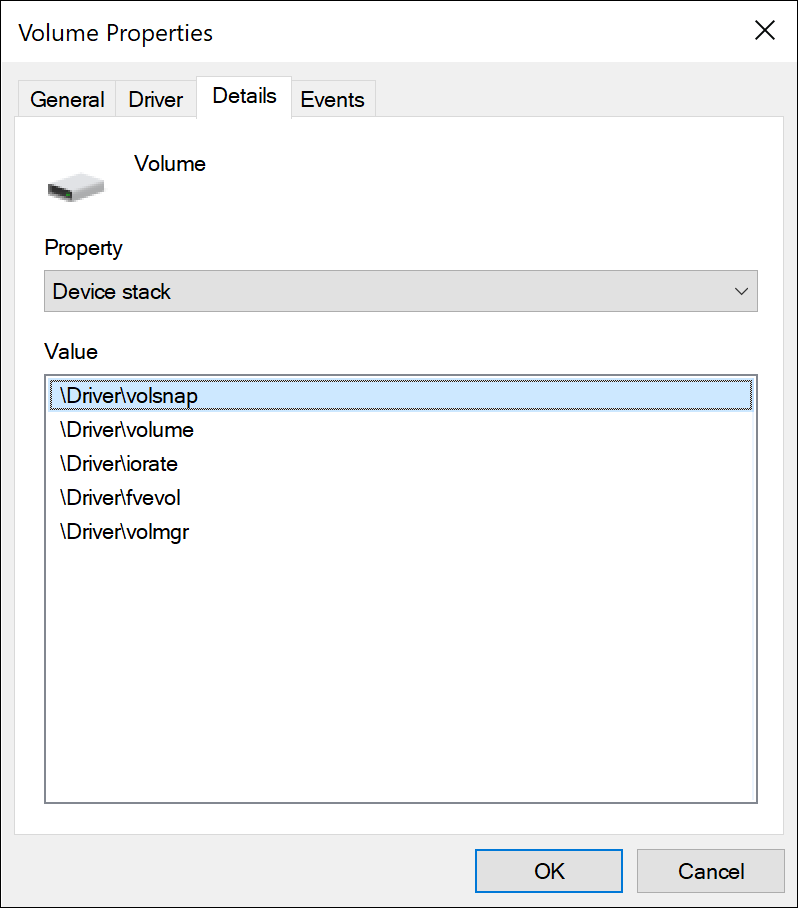
\includegraphics[scale=0.7]{../img/background.kerneldriver.devicestack.png}
	\caption[
		Example of a device stack for a storage volume
	]{
		Example of a device stack for a storage volume (Screenshot from device properties in Windows Device Manager). The official descriptions of the drivers listed in this example are, from top to bottom: ``Volume Shadow Copy driver'', ``Volume driver'', ``I/O rate control filter'', ``BitLocker Drive Encryption Driver'', and ``Volume Manager Driver''. As can be seen under the appropriate registry key\footnotemark, \texttt{fvevol} and \texttt{iorate} are lower filter drivers and \texttt{volsnap} is an upper filter driver. This leaves \texttt{volume} as the function driver and \texttt{volmgr} as the bus driver.
	}
	\label{fig:background.kerneldriver.devicestack}
\end{figure}
\footnotetext{\label{fn:background.kerneldriver.registryvolume} Later on in this section we will talk about the registry's role in driver management in more detail. See \autoref{fig:background.kerneldriver.registry} for what key to use and how the values stored under that key may look. \todo{ensure correct position}}

The device stack is built by the PnP manager during a process called \emph{device enumeration}. This happens at system boot or when resuming from hibernation, but it can also be triggered manually. During enumeration, the PnP manager constructs a so-called \emph{device tree} that captures the parent-child relationships of devices. A node in this tree represents a physical device and is appropriately called a \emph{device node}, or short \emph{devnode}. When a new device is discovered, its required drivers are loaded (if they have not already been loaded). The drivers are then informed about the new device, and can decide whether they want to be part of the device stack or not \cite{Yosifovich2017}.

For all the drivers of a device, the PnP manager creates objects that are used for managing and representing the relationships between the drivers. These objects form the device stack. They are also a form of device object, however they don't represent a real, physical device, but rather a virtual one. See \autoref{fig:background.kerneldriver.devnode} for an example device node and the objects it is made of. There are the following types of objects in a device node, ordered from bottom to top by their occurrence in a devnode \cite{Yosifovich2017}:
\begin{itemize}
	\item exactly one \emph{physical device object (PDO)}, created by the bus driver. It is responsible for the physical device interface.
	\item zero or more \emph{filter device objects (FiDOs)}, created by lower filter drivers (lower being relative to the FDO).
	\item exactly one \emph{functional device object (FDO)}, created by the device's function driver. It is responsible for the logical device interface.
	\item zero or more FiDOs, created by upper filter drivers.
\end{itemize}

This shows that filter drivers can be places either above the function driver (upper filter drivers) or between the function driver and the bus driver (lower filter drivers). These serve different purposes: ``In most cases, lower-level filter drivers modify the behavior of device hardware. For example, if a device reports to its bus driver that it requires 4 I/O ports when it actually requires 16 I/O ports, a lower-level, device-specific function filter driver could intercept the list of hardware resources reported by the bus driver to the PnP manager and update the count of I/O ports. Upper-level filter drivers usually provide added-value features for a device. For example, an upper-level device filter driver for a disk can enforce additional security checks.'' \cite{Yosifovich2017}

\begin{figure}[htb!]
	\center
	\begin{tikzpicture}
		\node[rect, fill=tYlow, from={0.2, 0.3 to 3.8, 7.1}] {};
		\node[rect, fill=tLblu, text width=5em] at (2, 6.4)  {\small FiDO};
		\node[rect, fill=tLblu, text width=5em] at (2, 5.5)  {\small FiDO};
		\node[rect, fill=tLblu, text width=5em] at (2, 4.6)  {\small FiDO};
		\node[rect, fill=tGren, text width=5em] at (2, 2.8)  {\small FiDO};
		\node[rect, fill=tGren, text width=5em] at (2, 1.9)  {\small FiDO};
		\node[rect, fill=tBlue, text width=7em, rounded corners=9pt] at (2, 3.7) {\small FDO};
		\node[rect, fill=tPink, text width=7em, rounded corners=9pt] at (2, 1)   {\small PDO};

		\draw[decorate, decoration={calligraphic brace, amplitude=10pt, mirror}, semithick] (0.2, 0.1) -- (3.8, 0.1) node[midway, yshift=-18pt] {\small Device node};

		\node[anchor=west] at (4, 6.4) {Upper Filter Driver 3};
		\node[anchor=west] at (4, 5.5) {Upper Filter Driver 2};
		\node[anchor=west] at (4, 4.6) {Upper Filter Driver 3};
		\node[anchor=west] at (4, 3.7) {Function driver};
		\node[anchor=west] at (4, 2.8) {Lower Filter Driver 2};
		\node[anchor=west] at (4, 1.9) {Lower Filter Driver 1};
		\node[anchor=west] at (4, 1)   {Bus driver};
	\end{tikzpicture}
	\caption[
		A device node and its device stack
	]{
		A device node and its device stack (modified after \cite{Yosifovich2017}). See \autoref{fig:background.kerneldriver.devicestack} for a concrete example of a device stack.
	}
	\label{fig:background.kerneldriver.devnode}
\end{figure}

As already hinted at in the description of \autoref{fig:background.kerneldriver.devicestack}, the registry is responsible for storing the information that governs driver loading. Both which drivers are loaded and the order they are loaded in are configured this way. Basically, it is described how exactly the device nodes should be built. \autoref{tbl:background.kerneldriver.registrykeys} lists the registry keys that, together with their subkeys, are relevant for the configuration. \todo{mention that \autoref{chap:ourapproach.final} explains adding the required registry entries via INF files}

\begin{table}[htb!]
	\center
	\small
	\def\arraystretch{1.25}
	\begin{NiceTabular}{lll}
	\CodeBefore
		\rectanglecolor{gray!30}{1-1}{1-3}
	\Body
		\hlineB{2}
		\textbf{Registry Key} & \textbf{Short Name} & \textbf{Description} \\
		\hlineB{1.5}
		\texttt{HKLM\textbackslash System\textbackslash CCS\textbackslash Enum}                        & Hardware key & Settings for known hardware devices \\
		\texttt{HKLM\textbackslash System\textbackslash CCS\textbackslash Control\textbackslash Class} & Class key    & Settings for device types           \\
		\texttt{HKLM\textbackslash System\textbackslash CCS\textbackslash Services}                    & Software key & Settings for drivers                \\
		\hlineB{2}
	\end{NiceTabular}
	\caption[
		Important registry keys for driver loading
	]{
		Important registry keys for driver loading \cite{Yosifovich2017}. Note that \texttt{CCS} stands for \texttt{CurrentControlSet}.
	}
	\label{tbl:background.kerneldriver.registrykeys}
\end{table}

The keys from \autoref{tbl:background.kerneldriver.registrykeys} each have different roles \cite{Yosifovich2017}:
\begin{itemize}
	\item The Hardware key configures driver loading for individual hardware devices. Its subkeys all follow the pattern of \texttt{<Enumerator>\textbackslash <Device ID>\textbackslash <Instance ID>}. The enumerator is the name of the responsible bus driver; the device ID identifies a particular type of hardware, e.g. a specific model from one manufacturer; and the instance ID distinguishes different devices with the same device ID, e.g. the device's location on the bus or its serial number. The most important values for each device are: \texttt{Service}, which contains the name of the device's function driver (this is used as a subkey in the Software key); \texttt{LowerFilters} and \texttt{UpperFilters}, which each contain an ordered list of lower and upper filter driver names, respectively; and \texttt{ClassGUID}, which identifies the device's class (this is used as a subkey in the Class key).
	\item The Class key contains class GUIDs\footnote{\label{fn:background.kerneldriver.guids} Globally Unique Identifiers, also known as Universally Unique Identifiers (UUIDs). See \href{https://tools.ietf.org/html/rfc4122}{RFC 4122} for more information.} as subkeys. The configuration stored here is similar to the subkeys of the Hardware key, but applies to a whole class of devices. For example, the lower and upper filters listed under the GUID for the ``Volume'' class are loaded for all volumes.
	\item The Software key contains relevant information about drivers, most importantly the \texttt{ImagePath} value, which stores the path to the driver's \texttt{.sys} file. The subkey that contains the values for a driver is the driver's name.
\end{itemize}

Examples of subkeys of each of these keys are shown in \autoref{fig:background.kerneldriver.registry}.

\begin{figure}[htb!]
	\center
	
	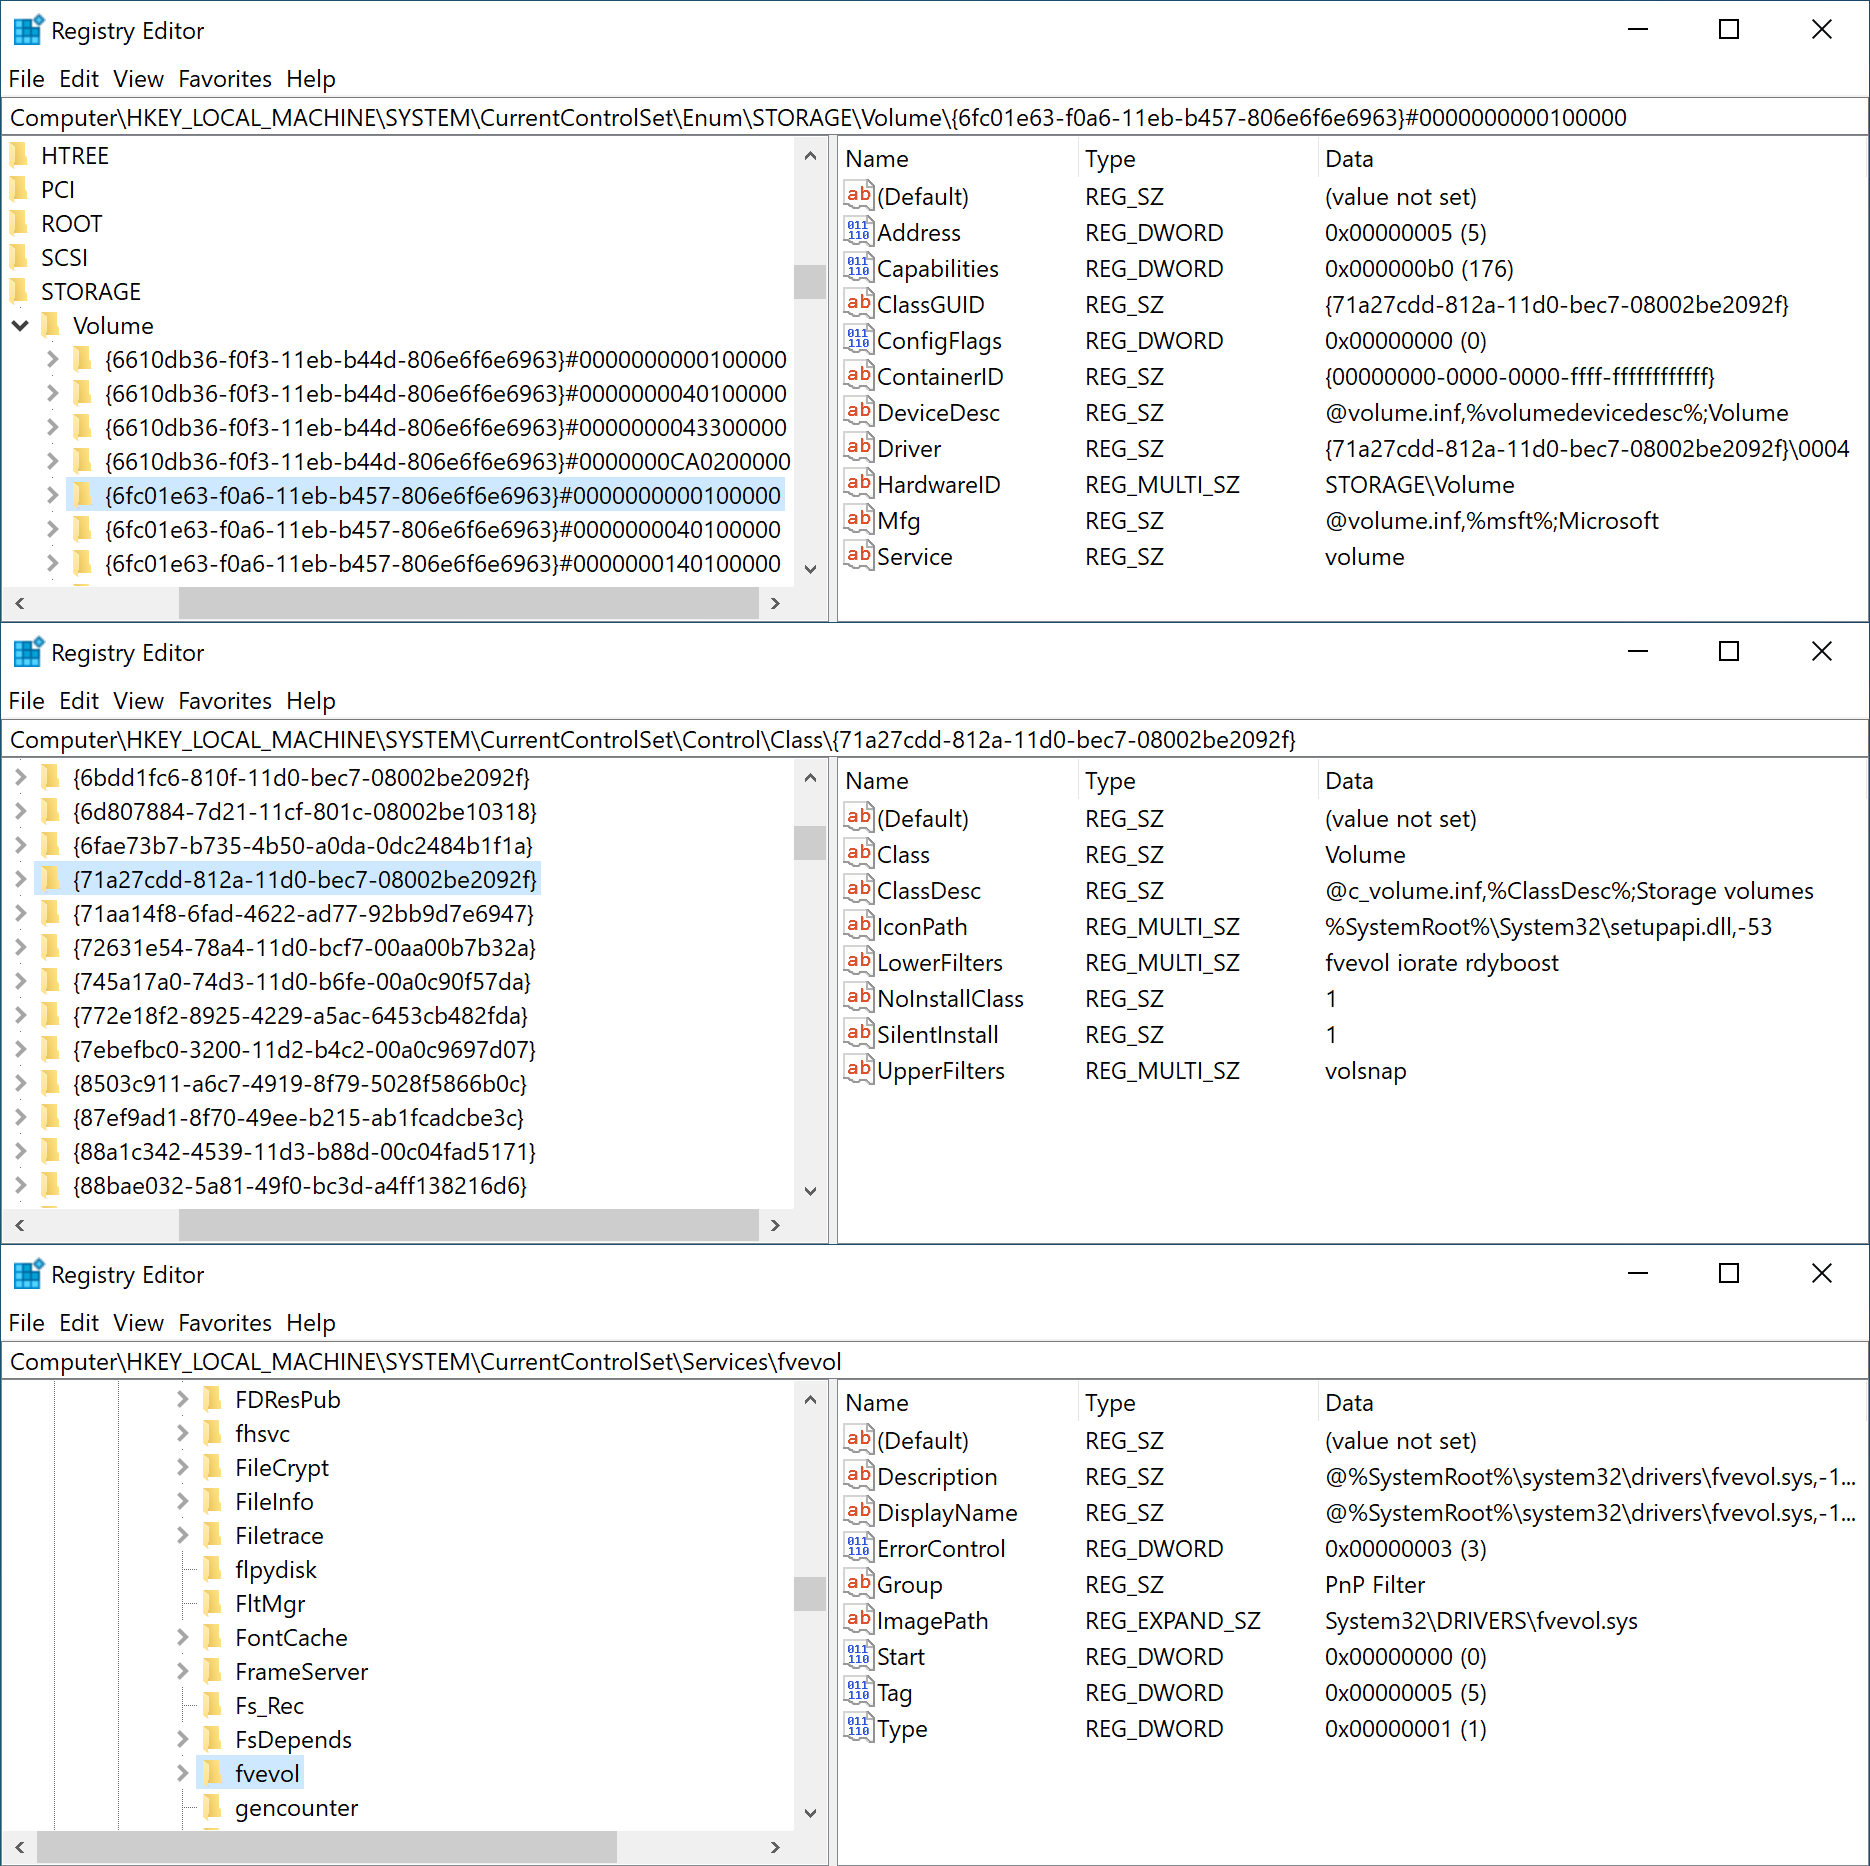
\includegraphics[scale=0.65]{../img/background.kerneldriver.registry.png}
	\caption[
		Example contents of a Hardware, Class, and Software subkey
	]{
		Example contents of a Hardware, Class, and Software subkey (Screenshots from the Windows Registry Editor). These are all relevant for the device whose device stack is shown in \autoref{fig:background.kerneldriver.devicestack}. As already partly discussed there, the configured values match the final device stack: the \texttt{Service} value under the Hardware subkey designates \texttt{volume} as the function driver; the drivers listed in the \texttt{LowerFilters} and \texttt{UpperFilters} values of the Class subkey are indeed loaded before or after \texttt{volume}, respectively (also note that they are loaded, from bottom to top, in the order listed; the \texttt{readyboost} driver does not appear in the device stack because it probably decided not to be part of it\footnotemark); the \texttt{ImagePath} under the Software subkey shows the path to one of the driver's \texttt{.sys} file.
	}
	\label{fig:background.kerneldriver.registry}
\end{figure}
\footnotetext{\label{fn:background.kerneldriver.rdyboost} Which makes sense, because it is responsible for the ReadyBoost technology, which is designed for SD cards and USB sticks, and not hard disk volumes. See \cite{Yosifovich2017} for more information on this technology. \todo{ensure correct position}}

\subsubsection{Important Concepts for Kernel Driver Development}
\label{chap:background.kerneldriver.concepts}
The goal of this section is to explain some concepts that are relevant when developing a file system filter driver. They concern execution contexts, memory access, and the kernel's I/O system.

The code of a driver can run in different thread contexts, depending on how it was called. This is mostly relevant for accessing memory, because the translation of virtual memory addresses into physical addresses depends on the thread context\footnote{\label{fn:background.kerneldriver.threadcontexts} This is an inherent property of the concept of virtual memory and applies not only to Windows, but to all virtual memory OSes, including Linux.}. We will discuss what exactly to keep in mind when accessing memory shortly. The three different contexts that driver code can run in are the following \cite{Yosifovich2017}:
\begin{itemize}
	\item when called to handle an I/O request initiated by a user thread, the driver code runs in this thread's context;
	\item when called by a OS component, e.g. the PnP manager, the driver code runs in the context of the calling system thread;
	\item when called via an interrupt, it is not possible to predict in which context the driver code will run. The context of whatever thread was currently executing when the interrupt arrived will be used. The interrupt may stem from hardware, for example when a device informs about available data, or from software, for example when a timer fires.
\end{itemize}
Note that, regardless of the context, the code always executes in kernel mode. When running in the context of a user mode thread, the CPU switches to kernel mode before running the driver code \cite{Yosifovich2017}.

Another important parameter of code execution is the so-called \emph{interrupt request level (IRQL)}. As the name suggests, this has something to do with interrupts, but for this thesis it suffices to talk about one important property of this numerical value: code running at a lower IRQL cannot interrupt code running at a higher IRQL. We will discuss the implications of this in a moment. The normal IRQL of the CPU is 0, also called \texttt{PASSIVE\_LEVEL}. This is also the only possible value when in user mode. Another possible value for kernel mode code, more or less the only other one non-device drivers (such as filter drivers) will come in contact with, is an IRQL of 2. This is known as \texttt{DISPATCH\_LEVEL}. We will present a concrete example of code that can run at \texttt{DISPATCH\_LEVEL} when talking about the I/O system. The important thing is that the kernel's thread scheduler runs at this IRQL. Because of the property mentioned earlier, this means that the scheduler cannot interrupt code running at \texttt{DISPATCH\_LEVEL}. The immediate consequences of this are \cite{Yosifovich2017}:
\begin{itemize}
	\item Synchronization objects that rely on the scheduler's support, such as semaphores or mutexes, no longer work. The problem is that when waiting on one of these objects, the thread goes to sleep. But the scheduler can't run, because that would mean interrupting the thread, and thus it can never wake up the thread again. Windows prevents this by checking the IRQL and crashing if the current IRQL has a value of 2.
	\item Page faults must not occur. Handling them requires a context switch, but for that the scheduler would need to work. Therefore, code at \texttt{DISPATCH\_LEVEL} can only access memory that is not currently paged to disk. This can be ensured by allocating the memory in a special pool which, by definition, always is resident in memory: the \emph{non-paged pool}\footnote{\label{fn:background.kerneldriver.pagedpool} There also exists an allocation pool without this special guarantee, called the \emph{paged pool}.}.
\end{itemize}
In general, when running at an IRQL of 2, every called function needs to be checked for the ability to be called at this level. The supported IRQL is documented for all WDK functions.

As mentioned before, access to memory in userspace generally requires special care. To be precise, the following problems can occur \cite{Yosifovich2017}:
\begin{itemize}
	\item Recall that the translation of user mode virtual addresses to physical addresses depends on the thread context. Referencing an address from a different context than it belongs to either leads to an access violation or accesses random data from another process.
	\item Userspace memory always has the risk of being paged out. Code running at an IRQL of 2 must ensure that this is not the case before accessing memory. As discussed before, page faults are illegal in this state.
\end{itemize}

One situation where a driver needs to access user memory is doing I/O, i.e. read or write operations. Because these are so common, the I/O manager presents a solution, namely the \emph{Buffered I/O} and the \emph{Direct I/O} modes \cite{Yosifovich2017}:
\begin{descitemize}
	\item[Buffered I/O] When using this mode, the I/O manager copies the data from the user buffer to a newly allocated kernel buffer from the non-paged pool (or vice versa, depending on whether it is a read or write operation). This means the driver does not have to care about accessing the user buffer at all and can just work with the kernel buffer. Because it was allocated from non-paged pool, no page fault can occur, and as a system space address, the kernel buffer address is valid in any thread context. See \autoref{fig:background.kerneldriver.bufferedio} for how this works when reading data. Buffered I/O is commonly used for small buffers (up to one page, or 4KB).
	\item[Direct I/O] In this mode, the I/O manager locks the user buffer in RAM, so that it cannot be paged out to disk. The driver can then create a mapping of the buffer in kernel memory and just use that, without any copying. To do so, the I/O manager provides the driver with a MDL, which stands for \emph{memory descriptor list}. It holds information about the physical memory occupied by the user buffer, and it is needed to map the buffer into system space. At this point, the buffer's physical memory is mapped twice: once into user memory, and once into kernel memory. Both mappings can be accessed at any IRQL, because the buffer cannot be paged out. However, while the user mapping is only valid in one thread context, the kernel mapping is always valid. After the operation has completed, the I/O manager removes the kernel mapping and unlocks the buffer. \autoref{fig:background.kerneldriver.directio} illustrates this process. Direct I/O is useful when using large buffers (larger than one page, or 4KB), because no copying is needed\footnote{\label{fn:background.kerneldriver.dma} It is also more suitable than buffered I/O for devices with direct memory access (DMA), ``because DMA is used to transfer data from a device to RAM or vice versa without CPU intervention -- but with buffered I/O, there is always copying done with the CPU, which makes DMA pointless.'' \cite{Yosifovich2017}}.
\end{descitemize}

\begin{figure}[htb!]
	\center
	\begin{tikzpicture}
		% PART 1
		\node[rectangle, fill=tBlue, from={0, 9 to 2.5, 10}] {\footnotesize User Buffer};
		\draw (0, 8) rectangle (2.5, 14);
		\draw (0, 11) -- (2.5, 11);
		\draw (0, 10) -- (2.5, 10);
		\draw (0, 9)  -- (2.5, 9);
		\node[anchor=north] at (1.25, 14) {\footnotesize Kernel Space};
		\node[anchor=south] at (1.25, 8)  {\footnotesize User Space};

		\draw[decorate, decoration={calligraphic brace, amplitude=5pt}, semithick] (-0.1, 9) -- (-0.1, 10) node[midway, anchor=east, xshift=-5pt] {\footnotesize $N$ bytes};

		\node[circ=1.2em] at (-1.5, 7.2) {\small 1};
		\node[anchor=west, align=left] at (-1.2, 7.2) {User client allocates buffer\\and invokes read operation};

		% PART 2
		\node[rectangle, fill=tOrng, from={7, 12 to 9.5, 13}] {\footnotesize Kernel Buffer};
		\node[rectangle, fill=tBlue, from={7, 9 to 9.5, 10}]  {\footnotesize User Buffer};
		\draw (7, 8) rectangle (9.5, 14);
		\draw (7, 11) -- (9.5, 11);
		\draw (7, 10) -- (9.5, 10);
		\draw (7, 9)  -- (9.5, 9);
		\draw (7, 12) -- (9.5, 12);
		\draw (7, 13) -- (9.5, 13);
		\node[anchor=north] at (8.25, 14) {\footnotesize Kernel Space};
		\node[anchor=south] at (8.25, 8)  {\footnotesize User Space};

		\draw[decorate, decoration={calligraphic brace, amplitude=5pt}, semithick] (6.9, 12) -- (6.9, 13) node[midway, anchor=east, xshift=-5pt] {\footnotesize $N$ bytes};
		\draw[decorate, decoration={calligraphic brace, amplitude=5pt}, semithick] (6.9, 9)  -- (6.9, 10) node[midway, anchor=east, xshift=-5pt] {\footnotesize $N$ bytes};

		\node[rectangle, fill=tGren, from={10.5, 10.5 to 13, 11.5}] {};
		\draw (10.5, 9.5) rectangle (13, 12.5);
		\node[anchor=north] at (11.75, 12.5) {\footnotesize RAM};
		\draw (10.5, 10.5) -- (13, 10.5);
		\draw (10.5, 11.5) -- (13, 11.5);
		\draw (9.5, 12) -- (10.5, 10.5);
		\draw (9.5, 13) -- (10.5, 11.5);

		\node[circ=1.2em] at (5.7, 7.2) {\small 2};
		\node[anchor=west, align=left] at (6.0, 7.2) {I/O manager allocates\\buffer in non-paged pool};

		% PART 3
		\node[rectangle, fill=tPink, from={0, 4 to 2.5, 5}] {\footnotesize Data};
		\node[rectangle, fill=tBlue, from={0, 1 to 2.5, 2}] {\footnotesize User Buffer};
		\draw (0, 0) rectangle (2.5, 6);
		\draw (0, 3) -- (2.5, 3);
		\draw (0, 4) -- (2.5, 4);
		\draw (0, 5) -- (2.5, 5);
		\draw (0, 1) -- (2.5, 1);
		\draw (0, 2) -- (2.5, 2);
		\node[anchor=north] at (1.25, 6) {\footnotesize Kernel Space};
		\node[anchor=south] at (1.25, 0) {\footnotesize User Space};

		\node[rectangle, fill=tPink, from={3.5, 2.5 to 6, 3.5}] {\footnotesize Data};
		\draw (3.5, 1.5) rectangle (6, 4.5);
		\node[anchor=north] at (4.75, 4.5) {\footnotesize RAM};
		\draw (3.5, 2.5) -- (6, 2.5);
		\draw (3.5, 3.5) -- (6, 3.5);
		\draw (2.5, 4) -- (3.5, 2.5);
		\draw (2.5, 5) -- (3.5, 3.5);

		\node[circ=1.2em] at (-0.85, -0.8) {\small 3};
		\node[anchor=west, align=left] at (-0.55, -0.8) {Driver writes data\\to kernel buffer};

		% PART 4
		\node[rectangle, fill=tPink, from={7, 4 to 9.5, 5}] {\footnotesize Data};
		\node[rectangle, fill=tPink, from={7, 1 to 9.5, 2}] {\footnotesize Data};
		\draw (7, 0) rectangle (9.5, 6);
		\draw (7, 3) -- (9.5, 3);
		\draw (7, 4) -- (9.5, 4);
		\draw (7, 5) -- (9.5, 5);
		\draw (7, 1) -- (9.5, 1);
		\draw (7, 2) -- (9.5, 2);
		\node[anchor=north] at (8.25, 6) {\footnotesize Kernel Space};
		\node[anchor=south] at (8.25, 0) {\footnotesize User Space};

		\draw[arrow] (9.5, 4.5) to [bend left=45] (9.5, 1.5);
		\node[anchor=west] at (10.15, 3) {\footnotesize Copy}; % node[midway] in a \draw with bend doesn't work

		\node[circ=1.2em] at (5.05, -0.8) {\small 4};
		\node[anchor=west, align=left] at (5.35, -0.8) {I/O manager copies data to user\\buffer and frees kernel buffer};
	\end{tikzpicture}
	\caption[
		Buffered I/O for a read operation
	]{
		Buffered I/O for a read operation (modified after \cite{Yosifovich2017}). For write operations, the copying is done before the driver is called to handle the request.
	}
	\label{fig:background.kerneldriver.bufferedio}
\end{figure}

\begin{figure}[htb!]
	\center
	\begin{tikzpicture}
		% PART 1
		\node[rectangle, fill=tBlue, from={0, 9 to 2.5, 10}] {\footnotesize User Buffer};
		\draw (0, 8) rectangle (2.5, 14);
		\draw (0, 11) -- (2.5, 11);
		\draw (0, 10) -- (2.5, 10);
		\draw (0, 9)  -- (2.5, 9);
		\node[anchor=north] at (1.25, 14) {\footnotesize Kernel Space};
		\node[anchor=south] at (1.25, 8)  {\footnotesize User Space};

		\draw[decorate, decoration={calligraphic brace, amplitude=5pt}, semithick] (-0.1, 9) -- (-0.1, 10) node[midway, anchor=east, xshift=-5pt] {\footnotesize $N$ bytes};

		\node[circ=1.2em] at (-1.9, 7.2) {\small 1};
		\node[anchor=west, align=left] at (-1.6, 7.2) {User client allocates buffer and\\invokes read or write operation};

		% PART 2
		\node[rectangle, fill=tOrng, from={7, 12 to 9.5, 13}] {};
		\node[rectangle, fill=tBlue, from={7, 9 to 9.5, 10}]  {\footnotesize User Buffer};
		\draw (7, 8) rectangle (9.5, 14);
		\draw (7, 11) -- (9.5, 11);
		\draw (7, 10) -- (9.5, 10);
		\draw (7, 9)  -- (9.5, 9);
		\draw (7, 12) -- (9.5, 12);
		\draw (7, 13) -- (9.5, 13);
		\node[anchor=north] at (8.25, 14) {\footnotesize Kernel Space};
		\node[anchor=south] at (8.25, 8)  {\footnotesize User Space};

		\draw[decorate, decoration={calligraphic brace, amplitude=5pt}, semithick] (6.9, 12) -- (6.9, 13) node[midway, anchor=east, xshift=-5pt] {\footnotesize $N$ bytes};
		\draw[decorate, decoration={calligraphic brace, amplitude=5pt}, semithick] (6.9, 9) -- (6.9, 10) node[midway, anchor=east, xshift=-5pt] {\footnotesize $N$ bytes};

		\node[rectangle, fill=tGren, from={10.5, 10.5 to 13, 11.5}] {};
		\draw (10.5, 9.5) rectangle (13, 12.5);
		\node[anchor=north] at (11.75, 12.5) {\footnotesize RAM};
		\draw (10.5, 10.5) -- (13, 10.5);
		\draw (10.5, 11.5) -- (13, 11.5);
		\draw (9.5, 12) -- (10.5, 10.5);
		\draw (9.5, 13) -- (10.5, 11.5);
		\draw (9.5, 9)  -- (10.5, 10.5);
		\draw (9.5, 10) -- (10.5, 11.5);

		\node[circ=1.2em] at (4.9, 7.2) {\small 2};
		\node[anchor=west, align=left] at (5.2, 7.2) {I/O manager locks buffer in RAM\\and maps it to system space};

		% PART 3
		\node[rectangle, fill=tPink, from={0, 4 to 2.5, 5}] {\footnotesize Data};
		\node[rectangle, fill=tPink, from={0, 1 to 2.5, 2}] {\footnotesize Data};
		\draw (0, 0) rectangle (2.5, 6);
		\draw (0, 4) -- (2.5, 4);
		\draw (0, 5) -- (2.5, 5);
		\draw (0, 1) -- (2.5, 1);
		\draw (0, 2) -- (2.5, 2);
		\draw (0, 3) -- (2.5, 3);
		\node[anchor=north] at (1.25, 6) {\footnotesize Kernel Space};
		\node[anchor=south] at (1.25, 0) {\footnotesize User Space};

		\node[rectangle, fill=tPink, from={3.5, 2.5 to 6, 3.5}] {\footnotesize Data};
		\draw (3.5, 1.5) rectangle (6, 4.5);
		\node[anchor=north] at (4.75, 4.5) {\footnotesize RAM};
		\draw (3.5, 2.5) -- (6, 2.5);
		\draw (3.5, 3.5) -- (6, 3.5);
		\draw (2.5, 4) -- (3.5, 2.5);
		\draw (2.5, 5) -- (3.5, 3.5);
		\draw (2.5, 1) -- (3.5, 2.5);
		\draw (2.5, 2) -- (3.5, 3.5);

		\node[circ=1.2em] at (-2.2, -0.8) {\small 3};
		\node[anchor=west, align=left] at (-1.9, -0.8) {Driver reads/writes from/to buffer\\using the system space address};
	\end{tikzpicture}
	\caption[
		Direct I/O for a read or write operation
	]{
		Direct I/O for a read or write operation (modified after \cite{Yosifovich2017}).
	}
	\label{fig:background.kerneldriver.directio}
\end{figure}

It is up to the driver to decide which I/O mode to use. Their choice is signalled to the I/O manager using a flag of their virtual device's object (the one that is part of the device node). This applies to all I/O operations, the exception being so-called \emph{device I/O control requests}. These are the Windows equivalent to Unix' \texttt{ioctl} syscall and are used to communicate with a device from user mode\footnote{\label{fn:background.kerneldriver.ioctls} An example is \texttt{IOCTL\_DISK\_GET\_DRIVE\_GEOMETRY}, which is used get the physical layout of a disk. See \url{www.ioctls.net} for a comprehensive (unofficial) list of almost all relevant control codes and the \href{https://docs.microsoft.com/en-us/windows/win32/api/ioapiset/nf-ioapiset-deviceiocontrol}{documentation for \texttt{DeviceIoControl} in \cite{Win32}} for information on how to use them.}. A device control code, specifying what exactly the user wants from the device, also defines the used I/O mode, and drivers must adhere to this \cite{Yosifovich2017}.

In situations where it is not too complicated, drivers can choose to handle the user buffer access completely by themselves. This mode is known as \emph{Neither I/O}. It has the advantage of zero overhead, because the I/O manager does no extra work. It does however increase the risk of bugs and possible security risks. See \cite{Yosifovich2017} for more information.

I/O operations have been mentioned a lot in this section. In the following paragraphs, the important details of the kernel's I/O system will be laid out.

Firstly, all I/O has a \emph{virtual file} as its target. This may be backed by a ``real'' file or by something different, like a device\footnote{\label{fn:background.kerneldriver.virtualfiles} This concept will be familiar to Linux users.}. This abstraction allows the I/O manager to only care about files, leaving the translation of file commands to device-specific operations to drivers \cite{Yosifovich2017}. 

Secondly, Windows' internal I/O system is packet-driven. Almost all I/O requests\footnote{\label{fn:background.kerneldriver.fastio} The exception is so-called \emph{Fast I/O}, which works differently \cite{Yosifovich2017}. It is not supported by our driver and will therefore not be covered.} travel through the different relevant parts of the system in the form of an \emph{I/O request packet (IRP)}, which contains all relevant information about the request. IRPs are allocated in non-paged pool, usually by the I/O manager\footnote{\label{fn:background.kerneldriver.irpallocation} The PnP or power manager also sometimes allocate IRPs \cite{Yosifovich2017}. For simplicity, we will write ``the I/O manager'' instead of ``the I/O, PnP, or power manager'' in the following paragraphs.}, but it is also possible for drivers to initiate I/O by creating an IRP. After an IRP's allocation and initialization, a pointer to it is passed to the driver that shall handle the request. The driver then performs its operation and returns the IRP to the I/O manager. It also reports whether it was able to complete the requested operation or whether further work by another driver needs to be done \cite{Yosifovich2017}.

An IRP holds a lot of information. For this thesis, it suffices to know about the following fields\footnote{\label{fn:background.kerneldriver.irp} See \cite{Yosifovich2017} and \href{https://docs.microsoft.com/en-us/windows-hardware/drivers/ddi/wdm/ns-wdm-_irp}{its documentation in \cite{Wdk}} for more details.} \cite{Yosifovich2017}:
\begin{itemize}
	\item a pointer to a MDL, if the driver uses the direct I/O method;
	\item a pointer to a system buffer, if the driver uses the buffered I/O method;
	\item information about an IRP's final status, if it has been completed;
	\item information about the IRP's stack locations, which will be explained momentarily.
\end{itemize}

In memory, the IRP is followed by one or more \emph{stack locations}, their count matching the number of drivers this IRP will pass through\footnote{\label{fn:background.kerneldriver.adjuststacksize} This value is known when allocating the IRP, because it is equal to the size of the device stack. In some scenarios, most of which involve the filter manager, an IRP might be sent over to a new device stack. This might necessitate readjusting the count of stack locations, if the new device stack has a different size than the one before \cite{Yosifovich2017}. We will discuss the filter manager in \autoref{chap:ourapproach.failed}.}. These stack locations are represented by \texttt{IO\_STACK\_LOCATION} structures, whose contents are shown and explained in \autoref{fig:background.kerneldriver.stacklocation}. Because the information about the request is split between the IRP and its stack location, drivers can modify the stack location parameters for the next driver, while keeping the current set of parameters. The original parameters may for example be useful in a completion routine \cite{Yosifovich2017}.

\begin{figure}[htb!]
	\center
	\small
	\begin{tikzpicture}
		\node[rectangle, fill=tPink,   from={0, 5.6 to 3, 6.4}] {\makecell{MajorFunction}};
		\node[rectangle, fill=tPink,   from={3, 5.6 to 6, 6.4}] {\makecell{MinorFunction}};
		\node[rectangle, fill=gray!30, from={0, 4.8 to 3, 5.6}] {\makecell{Flags}};
		\node[rectangle, fill=gray!30, from={3, 4.8 to 6, 5.6}] {\makecell{Control}};
		\node[rectangle, fill=tOrng,   from={0, 3.2 to 6, 4.8}] {\makecell{Parameters}};
		\node[rectangle, fill=tYlow,   from={0, 2.4 to 6, 3.2}] {\makecell{DeviceObject}};
		\node[rectangle, fill=tYlow,   from={0, 1.6 to 6, 2.4}] {\makecell{FileObject}};
		\node[rectangle, fill=tGren,   from={0, 0.8 to 6, 1.6}] {\makecell{CompletionRoutine}};
		\node[rectangle, fill=tLblu,   from={0, 0   to 6, 0.8}] {\makecell{Context}};

		\node[rect, fill=tBlue, from={7.5, 4.6 to 10.5, 5.4}] {\makecell{Read}};
		\node[rect, fill=tBlue, from={7.5, 3.6 to 10.5, 4.4}] {\makecell{Write}};
		\node[rect, fill=tBlue, from={7.5, 2.6 to 10.5, 3.4}] {\makecell{$\ldots$}};

		\draw (0, 0) rectangle (6, 6.4);
		\draw (3, 4.8) -- (3, 6.4);
		\draw (0, 5.6) -- (6, 5.6);
		\draw (0, 4.8) -- (6, 4.8);
		\draw (0, 3.2) -- (6, 3.2);
		\draw (0, 2.4) -- (6, 2.4);
		\draw (0, 1.6) -- (6, 1.6);
		\draw (0, 0.8) -- (6, 0.8);

		\draw[arrow] (6, 4) -> (7.5, 5);
		\draw[arrow] (6, 4) -> (7.5, 4);
		\draw[arrow] (6, 4) -> (7.5, 3);
	\end{tikzpicture}
	\caption[
		Layout of the \texttt{IO\_STACK\_LOCATION} structure
	]{
		Layout of the \texttt{IO\_STACK\_LOCATION} structure (modified after \cite{Yosifovich2017} using information from \cite{Wdk}). The \texttt{MajorFunction} field has one of 28 possible values, denoting the request type, e.g. \texttt{IRP\_MJ\_READ} or \texttt{IRP\_MJ\_WRITE}. \texttt{MinorFunction} is used to further specify the type for some of the major functions. We will not discuss \texttt{Flags} and \texttt{Control}, because they are only rarely relevant. The \texttt{Parameters} are ``a monstrous union of structures, each of which valid for a particular major function code or a combination of major/minor codes.'' They contain information further specifying the request, e.g. the byte offset when reading from a file. \texttt{DeviceObject} and \texttt{FileObject} are pointers to the related device and file objects. \texttt{CompletionRoutine} holds a pointer to a completion routine, which will be explained separately. \texttt{Context} is a driver-defined parameter passed to the completion routine.
	}
	\label{fig:background.kerneldriver.stacklocation}
\end{figure}

The I/O manager only initializes the first stack location before sending the IRP over to the driver at the top of the device stack. Each driver, except the lowest in the stack, is then responsible for initializing the stack location for the next driver. If a driver can complete an IRP and no other drivers need to be called, initializing the next stack location is of course not necessary. This initialization can be done in two ways \cite{Yosifovich2017}:
\begin{itemize}
	\item if no changes to the stack location are needed, the driver can ``skip'' the current stack location. This means that the next driver will receive the same parameters in its stack location as the current driver.
	\item if changes to the stack location need to be made, the driver can copy its stack location and modify the copy. Registering a completion routine (explained momentarily) counts as a change, and a driver must copy the stack location instead of skipping it in that case \cite{Wdk}.
\end{itemize}

The already mentioned completion routines are a way for drivers to intercept the flow of an IRP after its completion by another driver. Completion routines are called in the opposite order that they were registered in, i.e. those registered by lower drivers first. See \autoref{fig:background.kerneldriver.irpflow} for an example. In such a routine, a driver can check the status of the completed IRP and do necessary post-processing. It is even possibly to mark the IRP as uncompleted again and resend it down the stack \cite{Yosifovich2017}. Completion routines may run at an IRQL equal to \texttt{DISPATCH\_LEVEL} \cite{Wdk}.

\begin{figure}[htb!]
	\center
	\small
	\begin{tikzpicture}
		\node[rect, fill=gray!30, rounded corners=4pt, from={0, 7.2 to 4, 8.1}] (iomgr) {\small\makecell{I/O Manager}};
		\node[rect, fill=tBlue, text width=3em] at (-1.3, 6.7) {\small IRP};

		\node[rect, fill=tYlow, from={0.2, 0.3 to 3.8, 6.2}] {};
		\node[rect, fill=tLblu, text width=5em] at (2, 5.5)  {\small FiDO};
		\node[rect, fill=tLblu, text width=5em] at (2, 4.6)  {\small FiDO};
		\node[rect, fill=tGren, text width=5em] at (2, 2.8)  {\small FiDO};
		\node[rect, fill=tGren, text width=5em] at (2, 1.9)  {\small FiDO};
		\node[rect, fill=tBlue, text width=7em, rounded corners=9pt] at (2, 3.7) {\small FDO};
		\node[rect, fill=tPink, text width=7em, rounded corners=9pt] at (2, 1)   {\small PDO};

		\node[anchor=east] at (-0.2, 3.25) {\footnotesize Register completion routine};
		\node[anchor=east] at (-0.2, 1.45) {\footnotesize Register completion routine};
		\node[anchor=west] at (4.2, 3.25)  {\footnotesize Call completion routine};
		\node[anchor=west] at (4.2, 1.45)  {\footnotesize Call completion routine};

		\draw[arrow, shorten <=4pt] (iomgr.west) to [bend right=45] (0, 5.55);
		\draw[arrow] (0, 5.45) to [bend right=45] (0, 4.65);
		\draw[arrow] (0, 4.55) to [bend right=45] (0, 3.75);
		\draw[arrow] (0, 3.65) to [bend right=45] (0, 2.85);
		\draw[arrow] (0, 2.75) to [bend right=45] (0, 1.95);
		\draw[arrow] (0, 1.85) to [bend right=45] (0, 1.05);

		\draw[arrow] (4, 1.05) to [bend right=45] (4, 1.85);
		\draw[arrow] (4, 1.95) to [bend right=45] (4, 2.75);
		\draw[arrow] (4, 2.85) to [bend right=45] (4, 3.65);
		\draw[arrow] (4, 3.75) to [bend right=45] (4, 4.55);
		\draw[arrow] (4, 4.65) to [bend right=45] (4, 5.45);
		\draw[arrow, shorten >=4pt] (4, 5.55) to [bend right=45] (iomgr.east);
	\end{tikzpicture}
	\caption[
		Example IRP flow
	]{
		Example IRP flow (modified after \cite{Yosifovich2017}). The I/O manager sends an IRP down the device stack of a devnode. It first passes through two upper filter driverss and the function driver, with the latter registering a completion routine. It then passes through two lower filter drivers, with the second of those also registering a completion routing. After the bus driver completes the IRP, it travels back up the device stack. Because only the second lower filter driver and the function driver registered a completion routine, they are the only drivers that the IRP passes through on its way in this direction. The real path of the IRP is slightly more complex than shown in this figure, because normally the I/O manager takes care of routing the IRP from one driver to another \cite{Yosifovich2017}. It is also responsible for calling the completion routines \cite{Wdk}.
	}
	\label{fig:background.kerneldriver.irpflow}
\end{figure}

\subsubsection{Debugging Kernel Drivers}
\label{chap:background.kerneldriver.debugging}
Debugging a program in kernel mode is not as simple as debugging most user mode applications, because it is part of the OS. For example, stopping the execution, e.g. via break points, halts the whole computer. This section will introduce the tools necessary to debug a Windows kernel component.

There are two official programs for kernel debugging, kd and WinDbg. They are essentially equivalent, with the former being a console debugger and the latter a GUI debugger. Out of personal preference, we will use WinDbg in this thesis. \cite{Yosifovich2017} also uses WinDbg for exploring the internals of Windows, including a lot of screenshots and explaining many useful commands\footnote{\label{fn:background.kerneldriver.windbg} A list of common commands can also be found at \url{http://windbg.info/doc/1-common-cmds.html}.}. \todo{You can also find screenshots of WinDbg from the process of writing and}\\\todo{debugging our driver in \autoref{chap:ourapproach}.}

There are different ways to use WinDbg \cite{Yosifovich2017}:
\begin{itemize}
	\item as a debugger for user mode programs. It can be used for viewing and changing the contents of the program's memory, setting breakpoints, and other common debugging techniques. WinDbg can also attach to an already running process.
	\item to view a crash dump file that Windows created during a system crash\footnote{\label{fn:background.kerneldriver.crashdump} If enabled, the dump file is usually located at \texttt{C:\textbackslash Windows\textbackslash MEMORY.DMP}.}. This way one can find out more about what exactly caused the crash. The available commands are a subset of what would have been available if WinDbg had been debugging the operating system when the crash happened. For example, the call stack of the function that caused the crash can be displayed. \todo{say more explicitly what doesn't work in this mode}
	\item as a local kernel mode debugger. If booted in debug mode, WinDbg can attach to a currently running instance of Windows. Only a subset of the normally available commands can be used, and some advanced debugging such as setting breakpoints and dumping memory do not work. An alternative for local kernel debugging is the Sysinternals LiveKd program. This simulates a crash dump file using the contents of physical memory, and in contrast to WinDbg, it can dump memory.
	\item as a remote kernel mode debugger. This is the mode of operation with the most possibilities, but also the one that is the most complicated and expensive to set up. It requires two computers, a target computer, running the OS to be debugged, and a host computer, that uses WinDbg to debug the target. Because WinDbg does not run under the OS that is being debugged, the target computer can be completely halted and the current system state can be examined. The connection between the two computers can be via USB or the local network\footnote{\label{background.kerneldriver.vmdebugging} Debugging via network can also be used to debug a virtual machine, if the hardware for a second real computer is not available. See \href{https://docs.microsoft.com/en-us/windows-hardware/drivers/debugger/setting-up-network-debugging-of-a-virtual-machine-host}{the Windows Debugging Tools documentation} for more.}.
\end{itemize}

\todo{screenshot}